\documentclass[hyperref={pdfpagelabels=false}]{beamer}
\setbeamercolor{background canvas}{bg=white}
\usepackage{graphicx,lmodern,subfigure,ulem,color,graphicx,tikz,booktabs,natbib}
\usepackage{mathrsfs}
\usetheme{Warsaw}
%\definecolor{beamer@blendedblue}{rgb}{0.1,0.5,0.1}
%\definecolor{ForestGreen}{RGB}{60, 140, 60}
%\setbeamercolor{structure}{fg=beamer@blendedblue}
\setbeamertemplate{navigation symbols}{}
\setbeamertemplate{footline}[frame number]
\bibliographystyle{chicago}
\newcommand{\spitem}{\vspace{.3cm}\item}
\newcommand{\elas}{$E_{labor}$}
%\def \FigPath {Users\th3\Documents\Job_Market_Paper\Code\Figures} 
\DeclareMathOperator{\E}{\mathbb{E}}




\title{Uncertainty Shocks and Financial Shocks}
\author{Marco Brianti}
\institute{Boston College}
\date{October 2018}

\usetheme[
outer/progressbar=foot,
outer/numbering=none
]{metropolis}


\begin{document}
	
	\frame{\titlepage \begin{center} Dissertation Project \end{center} }
	

	
	
		\frame{\frametitle{Alternative Drivers of Economic Fluctuations}	
			
			\
			

			
Depth and duration of \textbf{financial crisis} 
\begin{itemize}
	\item[$\Rightarrow$] several challenges for standard business cycle models
\end{itemize}  
% who used traditional sources of BC fluctuations such as productivity shocks. In particular, those models together with those shocks were unable to explain important features specifically related to the financial crisis.

\

%In response to this limitation,		
New strands of literature arose proposing alternative shocks
\begin{enumerate}
	\item \textbf{Financial shocks} - Khan and Thomas (2013) JPE %among others Jerman and Quadrini (2012) AER, Christiano, Motto e Rostagno (2010) Working paper
	\item \textbf{Uncertainty shocks} - Bloom (2009) Econometrica %was the first to estimate the dynamic effect of uncertainty in a both an empirical and theoretical context 
	\end{enumerate}

\


\textit{The shocks that produced the recession were primarily associated with financial disruptions and heightened uncertainty}

\hfill  Stock and Watson (2012) 
%Stock and Watson (2012) comprehensive empirical anatomy of the Great recession
%The shocks that produced the recession were primarily associated with financial disruptions and heightened uncertainty		


	}

	\frame{\frametitle{Definitions}	
		
		\
		
%Important to define because both shocks are residuals from endogenouse proxy variables that depends on other structural shocks	
\textbf{Financial Shocks.} Unanticipated innovations to financial conditions orthogonal to any other known economic disturbance.
$$
F_t = g(s_t^Y) + s_t^F
$$
%A financial shock is an unexpected deterioration of the credit conditions - in general proxied by the credit spread - which cannot be explained by other economic forces as productivity or policies. How can we think about s^F? Following Gilchrist (2012) AER, as a change in the risk-bearing capacity of the lending sector which is not trigger by other shocks. So s^F is a measure of our ignorance of the capital market, but it is an imortant one because it represents independent changes in the credit conditions. 

\




\textbf{Uncertainty Shocks.} Innovations in the expected variance of future (traditional) shocks which cannot be explained by any current source of economic fluctuations.
$$
U_t = h(s_t^Y) + s_t^U
$$
%when agents observe large 1st-order shocks they may also use this information to update the distribution of future shocks implying a jump in uncertainty. However, this jump is endogenous to a large realized shock. How can we think about s^U? According to Nimark (2014) - AER and Forni, Gambetti, and Sala (2017) - WP, I interpret s^U as a signal regarding future states of the economy which implies changes in the variance of the distribution of future shocks.

	
}
	
	
	\frame{\frametitle{Empirical Challenge}	
		
		\
		
		\
		
			\begin{figure}
			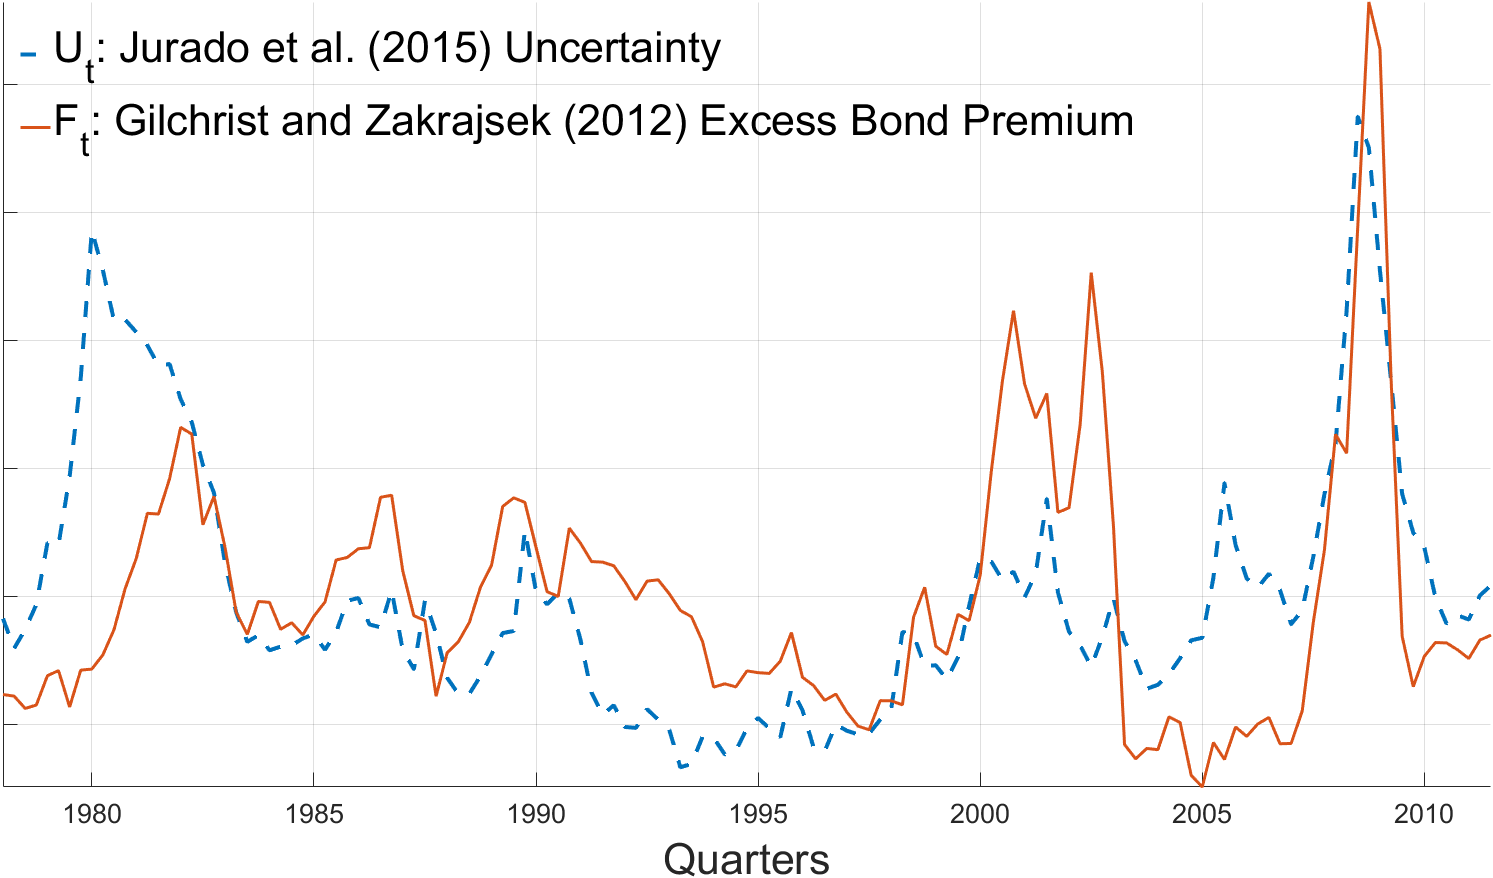
\includegraphics[scale=0.25]{Financial_Uncertainty}
			\label{fig:raw_data}
		\end{figure}
		
	}

	\frame{\frametitle{Empirical Challenge (cont.)}	
	
	Uncertainty shocks and financial shocks are deeply \textbf{confounded}.
	\begin{itemize}
		\item[$\Rightarrow$] correlation of raw series is above 0.5 
		\item[$\Rightarrow$] correlation of their \textbf{innovations} remains close to 0.5
	\end{itemize}

\


	Empirical literature did not succeed yet to disentangle these two exogenous sources due to:
\begin{enumerate}
	\item Simultaneity
	\begin{itemize}
		\item[$\Rightarrow$] Both types of variables are fast moving
	\end{itemize}	
	\item Effect on observables	
	\begin{itemize}
		\item[$\Rightarrow$] They have the same qualitative effects on prices and quantities
	\end{itemize}
\end{enumerate}
	
	
}





\frame{\frametitle{My contribution}
	
	I want to take a step back and show evidence and theory that financial and uncertainty shocks are \textbf{qualitative different}.
	
	
	\
	
	\	
	
	
	
	In particular, 
	
	
	\begin{enumerate}
		\item I argue that there exists a variable which responds differently to financial and uncertainty shocks. 	
		
		\item I provide a \textbf{new econometric tool} to identify two structural shocks when an internal instrument is available.
		
	\end{enumerate}
}

\frame{\frametitle{Roadmap}
	\Large{
		$ \ \ \ \ \ $ 1. \textbf{Cash Reserves}
		
		$ \ \ \ \ \ $ 2. Model
		
		$ \ \ \ \ \ $ 3. Empirical Strategy
		
		$ \ \ \ \ \ $ 4. Results
		
		$ \ \ \ \ \ $ 5. Conclusions
	}
}
	

\frame{\frametitle{Corporate Cash Holdings}
	
\textbf{Cash reserves} refer to money which a corporation keeps on hand to cover any emergency funding or short-term requirements. 

\

The typical U.S. large firm has cash equal to about 15\% of total assets.

\

Together with current cash flow is consider the most important \textbf{internal source of finance}.

\

Cash provides \textbf{unconditional liquidity} available at any time.


}


\frame{\frametitle{Cash Reserves and Financial Frictions}
	
	

	\begin{itemize}
	\item[1.] Financially constrained firms use cash as an \textbf{internal source of investment funding}.
	
	\hfill Kaplan and Zingales, 1997 QJE
\end{itemize}


		

	\begin{itemize}
	\item[2.] Financially constrained firms \textbf{store cash in good times} and \textbf{burn it in bad ones}.
	
	\hfill Almeida, Campello, Weisbach, 2004 JF 	
\end{itemize}
	
		

	\begin{itemize}
	\item[3.] After a negative credit supply shock firms \textbf{purposely burn cash} to \textbf{avoid investment cuts} due to credit constraints.
	
	\hfill Campello, Graham, Harvey, 2010 JFE
\end{itemize}

	

	\begin{itemize}
	\item[4.] At a country level, \textbf{cash-to-assets is positively correlated to credit-to-GDP}.
	
	\hfill Lins, Servaes, Tufano (2010) JFE
\end{itemize}

	

		
	
}

		\frame{\frametitle{Cash Reserves and Uncertainty}
				\begin{itemize}
				\item[1.] Financially constrained firm \textbf{holds more cash if cash flow is more volatile}.

\hfill Han and Qiu (2007) JCF
\end{itemize}

					\begin{itemize}
		\item[2.] Firms \textbf{increase their liquidity ratios when macroeconomic uncertainty increases}.
		
		\hfill Baum, Coglayan, Stephan, Talavera (2008) EM	
	\end{itemize}		

					\begin{itemize}
	\item[3.] Using UK data, they show that \textbf{cash is positively associated to higher uncertainty}.
	
	\hfill Bloom, Mizen, Smietanka (2018) WP	
\end{itemize}			
	


					\begin{itemize}
	\item[4.] In response to an \textbf{uncertainty shock}, firms \textbf{increase cash reserves}.
	
	\hfill Alfaro, Bloom, Lin (2018) NBER WP	
\end{itemize}	
	
}

\frame{\frametitle{Roadmap}
	\Large{
		$ \ \ \ \ \ $ 1. Cash Reserves
		
		$ \ \ \ \ \ $ 2. \textbf{Model}
		
		$ \ \ \ \ \ $ 3. Empirical Strategy
		
		$ \ \ \ \ \ $ 4. Results
		
		$ \ \ \ \ \ $ 5. Conclusions
	}
}
	
	
%\frame{\frametitle{Economic Intuition I}	
		
%To provide an economic intuition of the differential response of \textbf{cash holdings} to uncertainty and financial shocks, I present a properly augmented model in the spirit of 
%\begin{itemize}
	%\item Almeida, Campello, and Weisbach (2004)
	%\item Han and Qiu (2007)
%\end{itemize}

%\

%It is a simple representation of a dynamic setting where a credit-constrained profit-maximizing firm has a trade-off between present and future investment opportunities
		
%}

\frame{\frametitle{Setting}
	
	

\begin{itemize}
	\item[]
\begin{itemize}
     \item[Period 0] $ \ \ \ d_0 = y_0 + b_0 - i_0 - c$
	
	\
	
	
	\item[Period 1] $ \ \ \ d_1 = y_1 + b_1 - i_1 + c, \ \ \ $ where $ \ y_1 \sim F$
	
	\
	
	
	\item[Period 2] $ \ \ \ d_2 = g(I_0) - b_0 + h(I_1) - b_1$
\end{itemize}
\end{itemize}

\begin{eqnarray*}
	\begin{aligned}
\max_{\{ b_t,i_t,c \}_{t=0,1}} \ \ &\E \Big[  d_0 + d_1 + d_2     \Big| F  \Big] \\
\text{subject to} \ \ &b_t \leq (1 - \tau_t)i_t, \ \ \ t = 0,1 \\
&d_t \geq 0, \ \ \ t = 0,1,2
\end{aligned}
\end{eqnarray*}

\

\begin{center}
Financial shock: $\uparrow \tau_0$ $ \ \ \ \ $ vs $ \ \ \ \ $ Uncertainty shock: $\uparrow F$
\end{center}
	
}


\frame{\frametitle{Solution}
	
	Financially constrained firm: $I^*_t < I^{FB}_t$ for $t=0,1$
\begin{itemize}
	\item[$\Rightarrow$] $b_t = (1 - \tau_t)i_t \ \ $ for $ \ t=0,1$
	\item[$\Rightarrow$] $d_t = 0 \ \ $ for $ \ t=0,1$
\end{itemize}
which implies $I_0 = \frac{y_0 - c}{\tau_0}$ and $I_1 = \frac{y_1 + c}{\tau_1}$. Objective function is,
\begin{eqnarray*}
	\max_c g \bigg( \frac{y_0 - c}{\tau_0 } \bigg) - \frac{y_0 - c}{\tau_0 } +   \E \bigg[  h \bigg( \frac{y_1 + c}{\tau_1 } \bigg) - \frac{y_1 + c}{\tau_1 }   \bigg| F     \bigg]
	\end{eqnarray*}
and optimal condition for $c^*(\tau_0,F)$ is
\begin{eqnarray*}
\underbrace{g' \bigg( \frac{y_0 - c^*(\tau_0,F)}{\tau_0 } \bigg)}_{\text{Marginal Return of $I_0$}} = \underbrace{\E \bigg[  h' \bigg( \frac{y_1 + c^*(\tau_0,F)}{\tau_1 } \bigg)  \bigg| F  \bigg]}_{\text{$\E$ Marginal Return of $I_1$}}
\end{eqnarray*}

}

\frame{\frametitle{Comparative Statics}
	Given the Euler equation for cash $c$,
	\begin{eqnarray*}
		\underbrace{g' \bigg( \frac{y_0 - c^*(\tau_0,F)}{\tau_0 } \bigg)}_{\text{Marginal Return of $I_0$}} = \underbrace{\E \bigg[  h' \bigg( \frac{y_1 + c^*(\tau_0,F)}{\tau_1 } \bigg)  \bigg| F  \bigg]}_{\text{$\E$ Marginal Return of $I_1$}}
	\end{eqnarray*}

\
	
\textbf{Uncertainty shock}: $y_1 \sim Q$ which is mean-preserving spread in $F$
	\begin{enumerate}
	\item[$\Rightarrow$] $c^*(\tau_0,Q) > c^*(\tau_0,F)$ as long as $h'''(\cdot) > 0$
\end{enumerate}

\

\textbf{Financial shock}: $\tau_0^f > \tau_0$ which is a decrease in $b_0$
	\begin{enumerate}
	\item[$\Rightarrow$] $c^*(\tau_0^f,Q) < c^*(\tau_0,F)$ 
\end{enumerate}



}

\frame{\frametitle{Discussion and Testable Implications}
	\begin{eqnarray*}
	g' \bigg( \frac{y_0 - c^*(\tau_0,F)}{\tau_0 } \bigg) = \E \bigg[  h' \bigg( \frac{y_1 + c^*(\tau_0,F)}{\tau_1 } \bigg)  \bigg| F  \bigg]
\end{eqnarray*}


Taking into account \textbf{endogenous responses} of $\tau_0$ to $F$ or viceversa how can my identification assumption be interpreted?
\begin{itemize}
\item[] Financial shock $\Rightarrow$ firms perceive to need more liquidity today rather than tomorrow, use cash today

\item[] Uncertainty shock $\Rightarrow$ firms perceive to need more liquidity tomorrow rather than today, save cash for tomorrow
\end{itemize}

Uncertainty shocks look like \textbf{expected financial shocks} %Duchin (2010) JF
\begin{itemize}
	\item[$\Rightarrow$] This is a testable implication!
	\item[$\Rightarrow$] $corr(\iota_t^U, s_{t,t+1}^F) \geq 80\%$
\end{itemize}

}

\frame{\frametitle{Roadmap}
	\Large{
		$ \ \ \ \ \ $ 1. Cash Reserves
		
		$ \ \ \ \ \ $ 2. Model
		
		$ \ \ \ \ \ $ 3. \textbf{Empirical Strategy}
		
		$ \ \ \ \ \ $ 4. Results
		
		$ \ \ \ \ \ $ 5. Conclusions
	}
}



\frame{\frametitle{Penalty Functions (I)}

Penalty functions is a maximization problem where the importance of the constraint depends on some assumptions.

\

Consider the standard constrained maximization problem,
$$
\max_x f(x) \ \ \text{s.t} \ \ g(x) \geq 0
$$
a penalty function is an unconstrained maximization problem
$$
\max_x f(x) + H \big( g(x) \big) 
$$


$\Rightarrow$ Assumptions on $H(\cdot)$ determines the importance of $g(x)$.


}


\frame{\frametitle{Penalty Functions (II)}
	
Given $\max_x f(x) \ \ \text{s.t} \ \ g(x) \geq 0$, I assume $H(\cdot)$ to be linear,
$$
\max_x f(x) + \delta  g(x), \ \ \ \delta > 0
$$
$\Rightarrow$ the larger $\delta$, the more important $g(x)$

\

Applied to SVARs, PFA has the flavor of \textbf{sign restrictions} but with the advantage that the problem is \textbf{just identified}. 

\

\textbf{Shortcoming}: parameter $\delta$ is exogenously chosen making the identification strategy less credible.
	
	
}



\frame{\frametitle{Identification (I)}
	
	Given the reduced-form system $X_t = \textcolor{red}{B} X_{t-1} + \iota_t$ where 
	\begin{itemize}
		\item $X_t = [U_t \ \ F_t \ \ Y_t]'$ where $Y_t$ are macroeconomic variables.
		\item $\iota_t' \iota_t = \Sigma_{\iota}$
	\end{itemize}
	\textbf{Step 1}
	\begin{eqnarray*}
		\max_{\gamma_{U}} \ & \ \sum_{t=0}^K e'_U B^t \tilde{A}_0 \gamma_U + \delta e'_{C} \tilde{A}_0 \gamma_U \\
		\text{subject to} \ & \ \delta \geq 0 \ \ \text{and} \ \ \gamma_U \gamma_U' = 1
	\end{eqnarray*}
	\textbf{Step 2}
	\begin{eqnarray*}
		\max_{\gamma_{F}} \ & \ \sum_{t=0}^J e'_F B^t \tilde{A}_0 \gamma_F - \delta e'_{C} \tilde{A}_0 \gamma_F \\
		\text{subject to} \ & \ \delta \geq 0, \ \ \gamma_F \gamma_F' = 1 \ \ \text{and} \ \ \gamma_U \gamma_F' = 0
	\end{eqnarray*}
	where $\tilde{A}_0 \tilde{A}'_0 = \Sigma_{\iota}$ and $e_j$ is a selection vector of variable $j$.
	
}


\frame{\frametitle{Identification (I)}
	
	Given the reduced-form system $X_t = B X_{t-1} + \iota_t$ where 
	\begin{itemize}
		\item $X_t = [U_t \ \ F_t \ \ C_t \ \ Y_t]'$ 
		\item $\iota_t' \iota_t = \Sigma_{\iota}$
	\end{itemize}
	\textcolor{red}{\textbf{Step 1 - Uncertainty Shock}}
	\begin{eqnarray*}
		\max_{\gamma_{U}} \ & \ \sum_{t=0}^K e'_U B^t \tilde{A}_0 \gamma_U + \delta e'_{C} \tilde{A}_0 \gamma_U \\
		\text{subject to} \ & \ \delta \geq 0 \ \ \text{and} \ \ \gamma_U \gamma_U' = 1
	\end{eqnarray*}


An uncertainty shock maximizes its effect on uncertainty over the first $K$ quarters with penalty (merit) $\delta$ if cash is negative (positive) on impact.
	
}

\frame{\frametitle{Identification (I)}

Given the reduced-form system $X_t = B X_{t-1} + \iota_t$ where 
\begin{itemize}
\item $X_t = [U_t \ \ F_t \ \ Y_t]'$ where $Y_t$ are macroeconomic variables.
\item $\iota_t' \iota_t = \Sigma_{\iota}$
\end{itemize}
\textcolor{red}{\textbf{Step 2 - Financial Shock}}
\begin{eqnarray*}
	\max_{\gamma_{F}} \ & \ \sum_{t=0}^J e'_F B^t \tilde{A}_0 \gamma_F - \delta e'_{C} \tilde{A}_0 \gamma_F \\
	\text{subject to} \ & \ \delta \geq 0, \ \ \gamma_F \gamma_F' = 1 \ \ \text{and} \ \ \gamma_U \gamma_F' = 0
\end{eqnarray*}
A financial shock maximizes its effect on credit spread over the first $J$ quarters with penalty (merit) $\delta$ if cash is positive (negative) on impact.
	
}





\frame{\frametitle{Identification (I)}
	
	Given the reduced-form system $X_t = B X_{t-1} + \iota_t$ where 
	\begin{itemize}
		\item $X_t = [U_t \ \ F_t \ \ Y_t]'$ where $Y_t$ are macroeconomic variables.
		\item $\iota_t' \iota_t = \Sigma_{\iota}$
	\end{itemize}
	\textbf{Step 1 - Uncertainty Shock}
	\begin{eqnarray*}
		\max_{\gamma_{U}} \ & \ \sum_{t=0}^K e'_U B^t \tilde{A}_0 \gamma_U + \textcolor{red}{\delta} e'_{C} \tilde{A}_0 \gamma_U \\
		\text{subject to} \ & \ \delta \geq 0 \ \ \text{and} \ \ \gamma_U \gamma_U' = 1
	\end{eqnarray*}
	\textbf{Step 2 - Financial Shock}
	\begin{eqnarray*}
		\max_{\gamma_{F}} \ & \ \sum_{t=0}^J e'_F B^t \tilde{A}_0 \gamma_F - \textcolor{red}{\delta} e'_{C} \tilde{A}_0 \gamma_F \\
		\text{subject to} \ & \ \delta \geq 0, \ \ \gamma_F \gamma_F' = 1 \ \ \text{and} \ \ \textcolor{red}{\gamma_U \gamma_F' = 0}
	\end{eqnarray*}
	where $\tilde{A}_0 \tilde{A}'_0 = \Sigma_{\iota}$ and $e_j$ is a selection vector of variable $j$.
	
}

\frame{\frametitle{Identification (II)}

I suggest a \textbf{general approach} where $\delta$ is treated as an endogenous parameter chosen by the data.
\begin{itemize}
\item[$\Rightarrow$] Given the problem above, set $\delta$ such that $\gamma_U \gamma'_F = 0$
\end{itemize}

\begin{center}
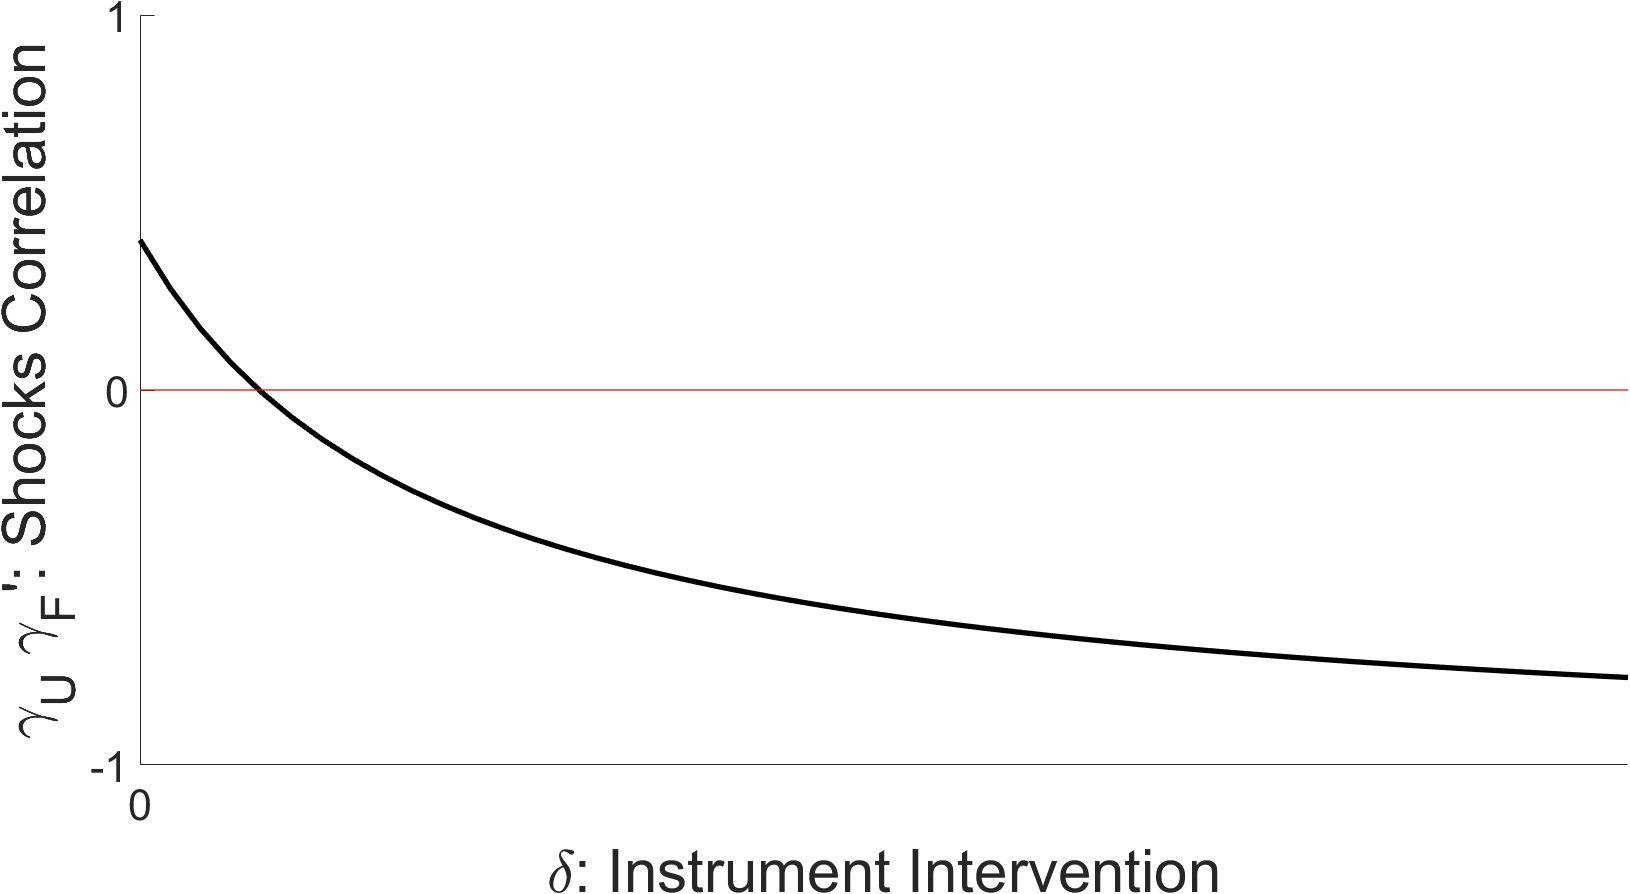
\includegraphics[scale=0.18]{fig_GPFA_intuition_figure_}
\end{center}

\textbf{Intuition.} Internal instrument intervention should be strong enough such that $\gamma_U \gamma_F' = 0$.

}

\frame{\frametitle{Roadmap}
	\Large{
		$ \ \ \ \ \ $ 1. Cash Reserves
		
		$ \ \ \ \ \ $ 2. Model
		
		$ \ \ \ \ \ $ 3. Empirical Strategy
		
		$ \ \ \ \ \ $ 4. \textbf{Results}
		
		$ \ \ \ \ \ $ 5. Conclusions
	}
}

\frame{\frametitle{Uncertainty Shock}

\begin{center}
	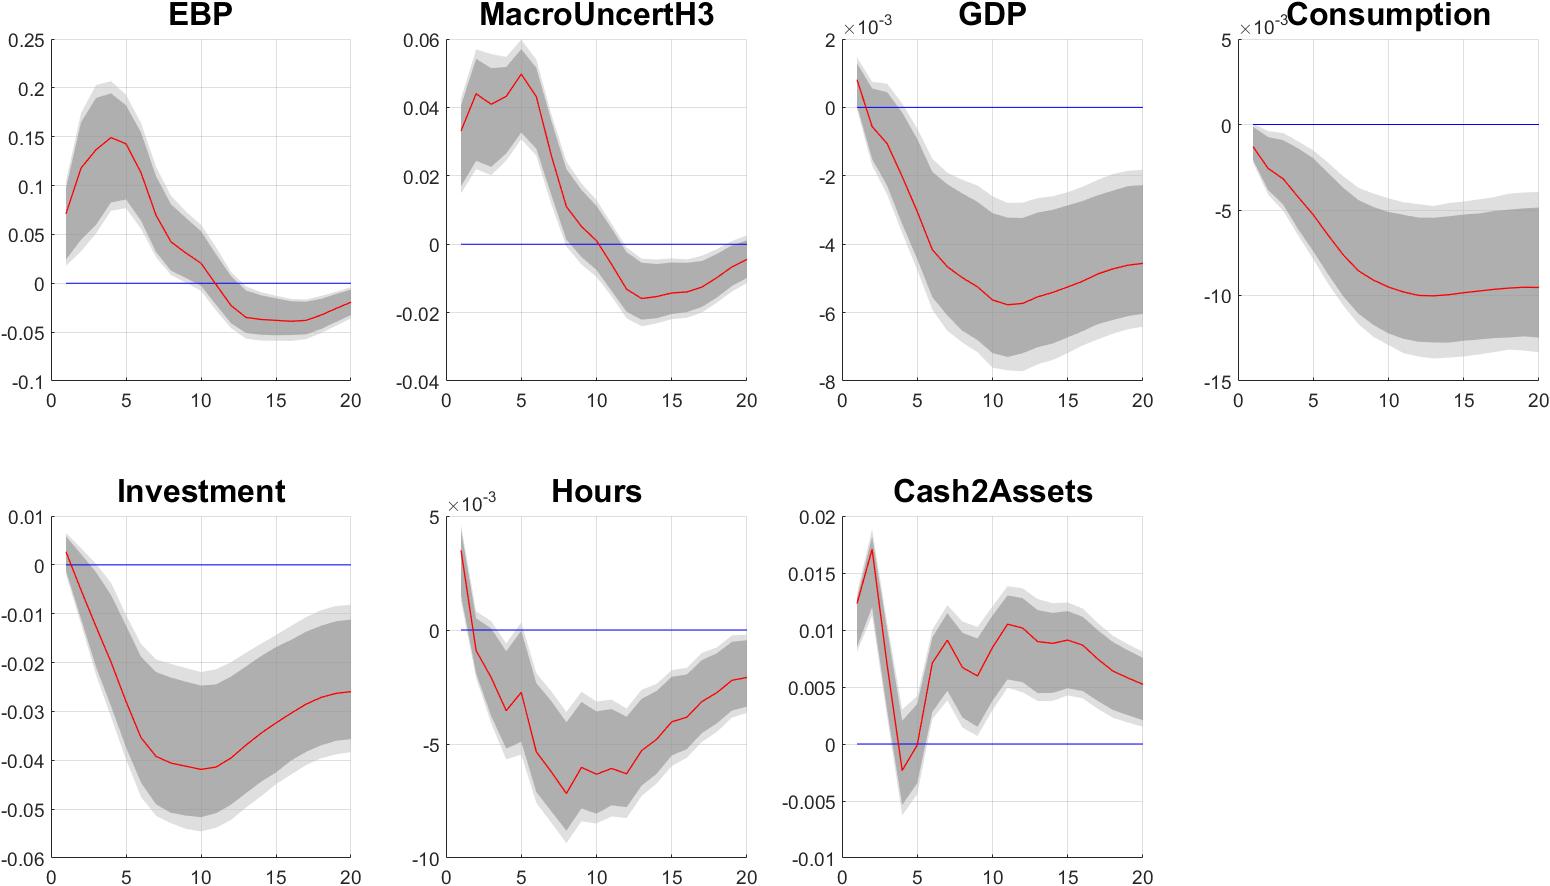
\includegraphics[scale=0.27]{fig_Uncertainty_Shock_GPFA_Compustat_3lags_03-Oct-2018_12_25_58}
\end{center}	

	
}

\frame{\frametitle{Financial Shock}
	
	\begin{center}
		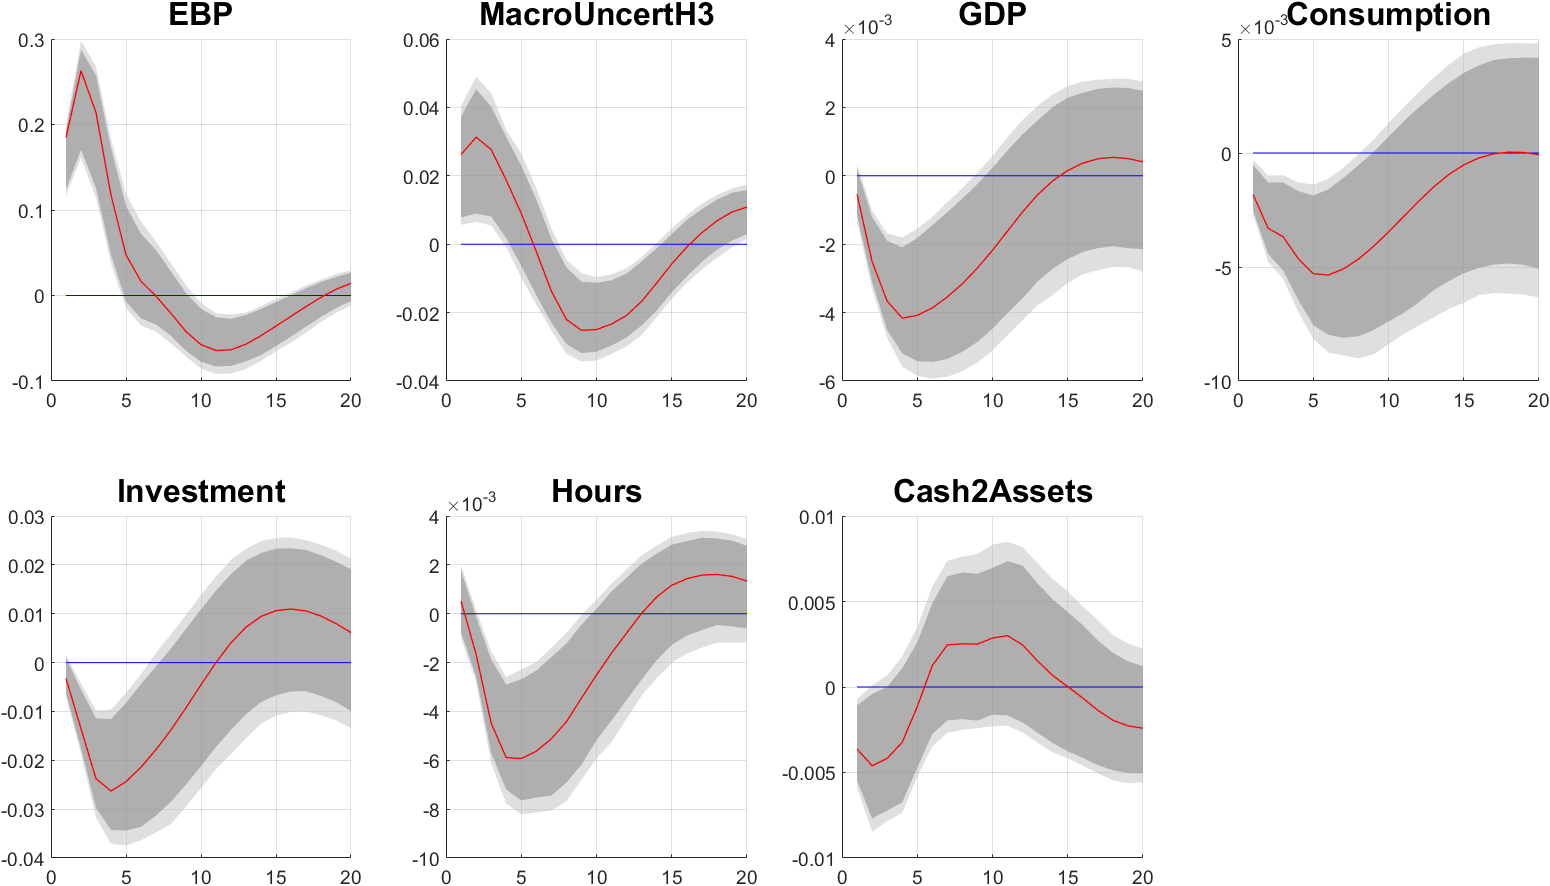
\includegraphics[scale=0.27]{fig_Financial_Shock_GPFA_Compustat_3lags_03-Oct-2018_12_26_00}
	\end{center}	
		
}



\frame{\frametitle{Variance Explained}
	
	\begin{center}
		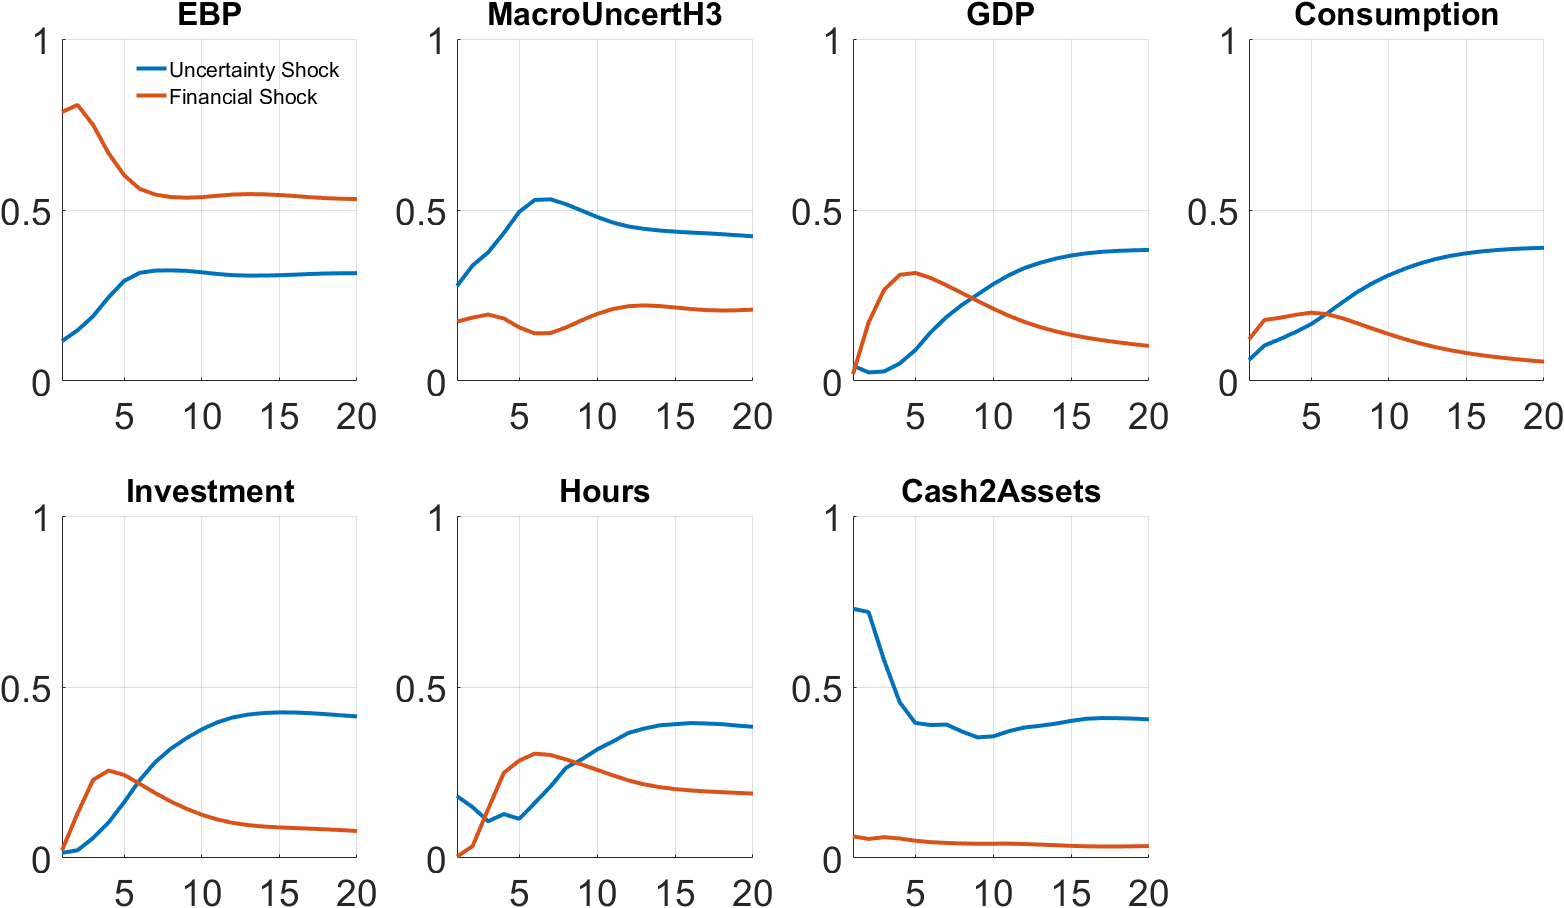
\includegraphics[scale=0.27]{fig_var_dec_vardec_GPFA_Compustat_3lags_03-Oct-2018_12_37_32}
	\end{center}	
	
}

\frame{\frametitle{Roadmap}
	\Large{
		$ \ \ \ \ \ $ 1. Cash Reserves
		
		$ \ \ \ \ \ $ 2. Model
		
		$ \ \ \ \ \ $ 3. Empirical Strategy
		
		$ \ \ \ \ \ $ 4. Results
		
		$ \ \ \ \ \ $ 5. \textbf{Conclusions}
	}
}

\frame{\frametitle{Conclusions}
	
\
	
Cash can be used as an internal instrument to simultaneously identify uncertainty and financial shocks

\

GPFA seems to be able to use internal instruments to fully disentangle two confounded shocks

\

Both shocks have a remarkable effect on aggregate variables 

\

Financial shocks have larger effect in the short run while uncertainty shocks in the medium run

}

















\end{document}